\begin{figure*}[t]
  \centering
  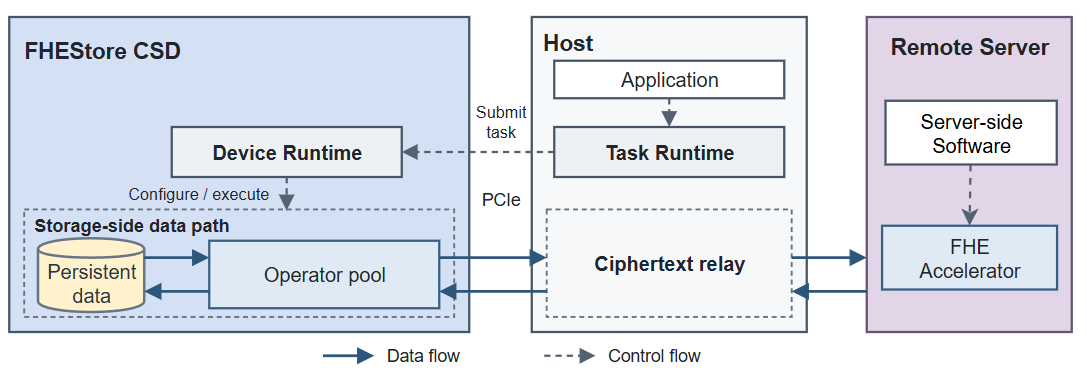
\includegraphics[width=\textwidth]{figures/fhestore-overview-v5/fhestore-overview.png}
  \caption{System overview of FHEStore. The CSD and host coordinate storage-side processing and ciphertext handoff; the remote server provides homomorphic evaluation through an FHE accelerator. PCIe connects the CSD to the host, which relays ciphertexts to and from the server over a network. Blue solid arrows denote data flow; gray dashed arrows denote control flow.}
  \Description{The CSD contains a device runtime and a storage-side data path with persistent data and an operator pool. The host contains an application, a task runtime, and a ciphertext relay. The remote server contains server-side software and an FHE accelerator. The host submits tasks over PCIe to the device runtime, which configures storage-side execution. Ciphertexts flow from the CSD operator pool through the host relay to the remote accelerator and return along the same route.}
  \label{fig:fhestore-overview}
\end{figure*}
